\chapter{Knowledge}
\label{cha:knowledgei}

\section{Prerequisites}

This section will introduce some important knowledges, including sigmoid function, Bayes Formula, Huffman code, etc.

\subsection{Sigmoid Function}

Sigmoid function is a common kind of active function, the definition is

$$ \sigma(x) = \frac{1}{1+e^{-x}}, $$

The domain is $(-\infty, \infty)$, the range is $(0,1)$.

\begin{figure}[H]
\centering
\begin{minipage}{.4\textwidth}
  \centering
	\fbox{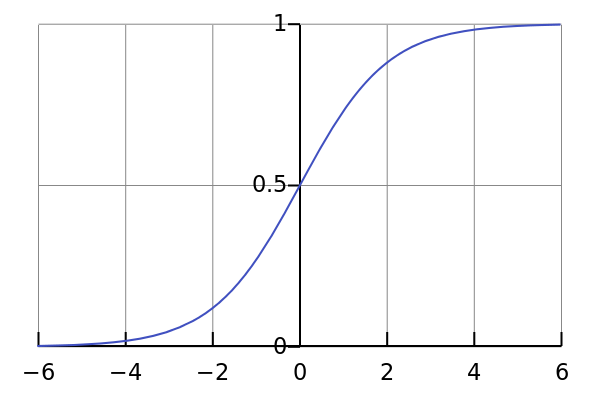
\includegraphics[width=0.95\textwidth]{sigmoid} }
	\caption{Sigmoid Function}
	\label{fig:sigmoid}
\end{minipage}
\end{figure}

Sigmoid function has the \textbf{derivative function} as following:

$$ \sigma^\prime(x) = \sigma(x)[1-\sigma(x)], $$

Thus, the \textbf{derivative functions} of $\mathrm{log}\sigma(x)$ and $\mathrm{log}(1-\sigma(x))$ are respectively

$$ [\mathrm{log}\sigma(x)]^\prime = 1-\sigma(x), \ [\mathrm{log}(1-\sigma(x))]^\prime = -\sigma(x), $$

\subsection{Logistic Regression}

Binary classification is a very common task, e.g. , if an email is spam, if a customer is a potential customer, if a online transaction fraud, etc. 

%--------------------------------------------------------------------------------------------------------------------------------%

\section{Skip-gram model}


\subsection{Softmax function}


\subsection{Hierarchical Softmax}


\subsection{Negative Sampling}

